\documentclass[pdflatex,sn-basic]{sn-jnl}

\usepackage{amsmath}
\usepackage{amssymb}
\usepackage{amsfonts}
\usepackage{amsthm}
\usepackage{mathrsfs}
\usepackage{multirow}
\usepackage{booktabs}
\usepackage{tabularx}
\usepackage{xcolor}
\usepackage{textcomp}
\usepackage{manyfoot}
\usepackage{algorithm}
\usepackage{algorithmicx}
\usepackage{algpseudocode}
\usepackage{listings}
\usepackage[title]{appendix}
\usepackage{url}
\graphicspath{{figures/}}

% Generated by paper/scripts/build_paper_assets.py. Do not edit by hand.
\newcommand{\MainGraphClusters}{20}
\newcommand{\InteractionP}{0.488}
\newcommand{\InteractionEffectRangePP}{30}
\newcommand{\StudyModels}{5}
\newcommand{\StudyMainPairs}{100}
\newcommand{\StudyMainBaseCorrect}{73}
\newcommand{\StudyMainDistCorrect}{45}
\newcommand{\StudyMainDeltaPP}{-28.0}
\newcommand{\StudyMainCILowPP}{-41.0}
\newcommand{\StudyMainCIHighPP}{-15.0}
\newcommand{\StudyMainSignFlipP}{0.0011}
\newcommand{\StudyBaselineOnly}{34}
\newcommand{\StudyDistractorOnly}{6}
\newcommand{\StudyMainPositiveGraphs}{2}
\newcommand{\StudyMainZeroGraphs}{4}
\newcommand{\StudyMainNegativeGraphs}{14}
\newcommand{\StudyASPP}{+26.0}
\newcommand{\StudyASPCILowPP}{+12.7}
\newcommand{\StudyASPCIHighPP}{+38.7}
\newcommand{\StudyASPSignFlipP}{0.0039}
\newcommand{\StudyASPPositiveGraphs}{11}
\newcommand{\StudyASPZeroGraphs}{2}
\newcommand{\StudyASPNegativeGraphs}{2}
\newcommand{\ASPRangeLowPP}{+20.0}
\newcommand{\ASPRangeHighPP}{+46.7}
\newcommand{\MiniMaxASPP}{+46.7}
\newcommand{\MiniMaxASPLowPP}{+23.3}
\newcommand{\MiniMaxASPHighPP}{+70.0}
\newcommand{\MiniMaxASPHolmP}{0.0342}
\newcommand{\DeepSeekBaseCorrect}{20}
\newcommand{\DeepSeekBaseTrials}{20}
\newcommand{\DeepSeekDistCorrect}{14}
\newcommand{\DeepSeekDistTrials}{20}
\newcommand{\DeepSeekDeltaPP}{-30.0}
\newcommand{\DeepSeekDeltaLowPP}{-50.0}
\newcommand{\DeepSeekDeltaHighPP}{-10.0}
\newcommand{\DeepSeekMcNemarP}{0.0312}
\newcommand{\DeepSeekHolmP}{0.1250}
\newcommand{\KimiBaseCorrect}{13}
\newcommand{\KimiBaseTrials}{20}
\newcommand{\KimiDistCorrect}{7}
\newcommand{\KimiDistTrials}{20}
\newcommand{\KimiDeltaPP}{-30.0}
\newcommand{\KimiDeltaLowPP}{-55.0}
\newcommand{\KimiDeltaHighPP}{-5.0}
\newcommand{\KimiMcNemarP}{0.0703}
\newcommand{\KimiHolmP}{0.2109}
\newcommand{\GLMBaseCorrect}{7}
\newcommand{\GLMBaseTrials}{20}
\newcommand{\GLMDistCorrect}{5}
\newcommand{\GLMDistTrials}{20}
\newcommand{\GLMDeltaPP}{-10.0}
\newcommand{\GLMDeltaLowPP}{-35.0}
\newcommand{\GLMDeltaHighPP}{+15.0}
\newcommand{\GLMMcNemarP}{0.6875}
\newcommand{\GLMHolmP}{0.6875}
\newcommand{\MiniMaxBaseCorrect}{16}
\newcommand{\MiniMaxBaseTrials}{20}
\newcommand{\MiniMaxDistCorrect}{8}
\newcommand{\MiniMaxDistTrials}{20}
\newcommand{\MiniMaxDeltaPP}{-40.0}
\newcommand{\MiniMaxDeltaLowPP}{-65.0}
\newcommand{\MiniMaxDeltaHighPP}{-15.0}
\newcommand{\MiniMaxMcNemarP}{0.0215}
\newcommand{\MiniMaxHolmP}{0.1074}
\newcommand{\QwenBaseCorrect}{17}
\newcommand{\QwenBaseTrials}{20}
\newcommand{\QwenDistCorrect}{11}
\newcommand{\QwenDistTrials}{20}
\newcommand{\QwenDeltaPP}{-30.0}
\newcommand{\QwenDeltaLowPP}{-60.0}
\newcommand{\QwenDeltaHighPP}{-5.0}
\newcommand{\QwenMcNemarP}{0.1094}
\newcommand{\QwenHolmP}{0.2188}


\begin{document}

\title[The Wrong Tool Looks Right]{The Wrong Tool Looks Right: Auditing Executable Goal-Irrelevant Tools in Multi-Step Tool Use}

\author*[1,2,3]{\fnm{Nianyi} \sur{Wang}}
\email{livingsailor@gmail.com; ORCID: 0000-0003-2587-1438}
\affil*[1]{\orgdiv{School of Mathematics and Computer Science},
\orgname{Northwest Minzu University},
\orgaddress{\city{Lanzhou}, \country{China}}}
\affil[2]{\orgdiv{Key Laboratory of Linguistic and Cultural Computing of
Ministry of Education}, \orgname{Northwest Minzu University},
\orgaddress{\city{Lanzhou}, \country{China}}}
\affil[3]{\orgdiv{Gansu Provincial Engineering Research Center of Multi-modal
Artificial Intelligence}, \orgname{Northwest Minzu University},
\orgaddress{\city{Lanzhou}, \country{China}}}

\abstract{A multi-step tool-using agent can fail after calls that are individually
valid. An executable goal-irrelevant tool may run and return a real value, yet
that value can violate the dependency required by a later tool. Comparisons based
on tool count conflate candidate-set size, connectivity, type compatibility, and
runtime execution. We present A3D, an audit system that holds the required
dependency task fixed, constructs equal-count tool-availability conditions, and
derives a first decisive error from saved calls. Across 20 shared depth-three
graphs and five API-served model aliases, five executable goal-irrelevant tools
were associated with a secondary, descriptive panel-level mean paired reduction
in exact success of
\StudyMainDeltaPP{} percentage points (graph-cluster 95\% CI
[\StudyMainCILowPP, \StudyMainCIHighPP] percentage points; sign-flip
p=\StudyMainSignFlipP). All model-specific point estimates were negative,
although none survived Holm correction as separate model-level tests.
Equal-count disconnected and connected-incompatible controls showed no
consistent loss of comparable magnitude; the study-level average separation
from these controls was \StudyASPP{} percentage points (95\% CI
[\StudyASPCILowPP, \StudyASPCIHighPP]). A 10-graph sealed probe directionally
implicated execution but remained exploratory. Rule-derived traces shifted
toward irrelevant calls and premature final answers, and simple reminders or
tool hiding did not improve success. These results position A3D as a
trace-level audit for depth-three tool-use reliability, not as a model ranking
or a validated repair method.}

\keywords{large language models, tool-use agents, function calling, executable goal-irrelevant tools, reliability evaluation, tool-call traces}

\maketitle

\section{Introduction}

Consider a task that requires four tools. The first returns a value that the
second must use, and the chain continues until the target is computed. Now add
five extra tools to the environment. One is connected to the current state,
accepts the available input type, can run, and is not in the required tool
chain. The model calls it. The call succeeds and returns a real value \(z\), but
the next required tool expects the output of the first required call, not \(z\).
Every individual call is valid. The trajectory is not.

We call a tool that can run but is not in the required tool chain an
\emph{executable goal-irrelevant tool}. We use ``tool'' and ``function''
interchangeably because each exposed tool is a callable function.

This is the failure that the paper studies. A high-level success rate records
the wrong final answer but does not show how the model left the required path.
Comparing a task with no extra tools to one with five extra tools is also
ambiguous, because the extra tools change several things at once: their number,
their connections, their argument types, and whether they can run. A decrease in
success may therefore come from the number of choices, from the tool graph, or
from a plausible but unusable branch.

We use \emph{tool usability} to refer only to properties visible at execution:
whether a tool is connected to the current state, whether its types match, and
whether it can run. Goal relevance is a separate question. A connected,
type-compatible tool can be fully usable and still be wrong for the task.
Throughout the paper, \emph{exact success rate} is the proportion of trials
whose final answer matches the program-computed target.

\begin{figure}[htbp]
\centering
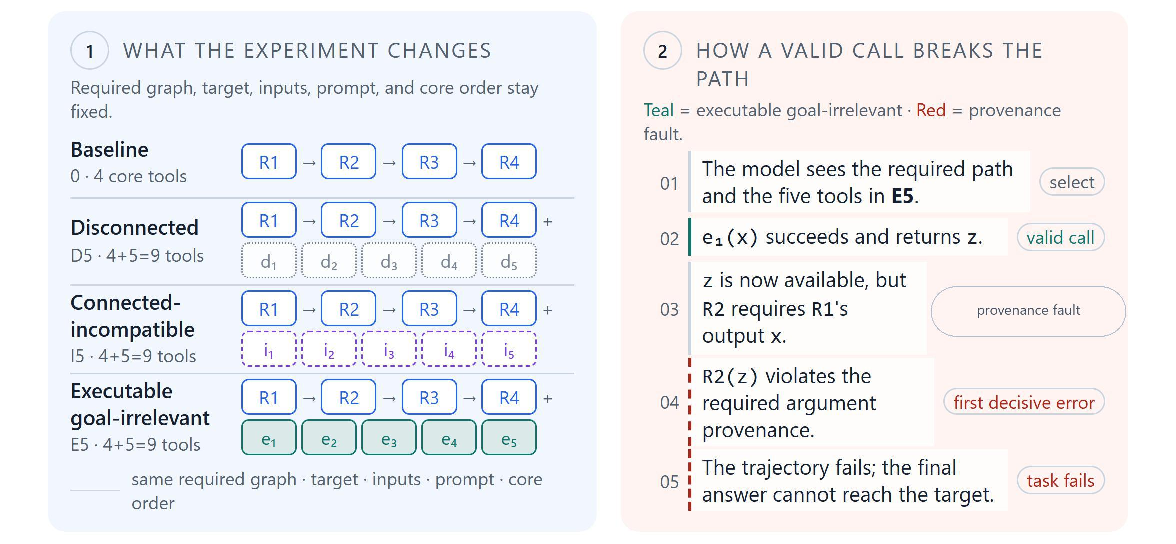
\includegraphics[width=\linewidth]{figure1_valid_call_invalid_path_v0124.pdf}
\caption{\textbf{A valid tool call can still break the task.} Left: the required
graph, target, inputs, prompt, and core order stay fixed while five extra tools
vary from disconnected to connected-incompatible to executable goal-irrelevant.
Right: a connected, type-compatible executable goal-irrelevant tool \(G_1\)
runs and returns \(z\). The call itself is valid, but \(R_2\) expects the output
of \(R_1\), not \(z\), so the trajectory cannot reach the target. The
argument-provenance violation at \(R_2\) is the first decisive error. Teal
marks the executable goal-irrelevant call and red marks the provenance fault.
The trace is illustrative rather than a reconstruction of one trial.}
\label{fig:wrong-tool}
\end{figure}

Figure~\ref{fig:wrong-tool} separates three levels of validity that are often
collapsed in tool-use evaluation. A call can be \emph{locally valid} when it can
execute, \emph{path-valid} when it preserves the required dependency provenance,
and \emph{finally valid} when the answer reaches the program-computed target.
The example is locally valid and finally invalid; the decisive failure is the
broken path. Endpoint benchmarks measure API selection, argument construction,
planning, and multi-tool execution
\citep{li2023apibank,qin2023toolllm,patil2023gorilla,shen2024taskbench}, but a
final score alone does not distinguish these levels or show where the path first
failed.

FuncBenchGen already provides hidden function-dependency graphs and
type-compatible extra tools \citep{maekawa2025funcbenchgen}. We do not claim those
mechanisms as new. The missing measurement is a counterfactual comparison in
which the required task is fixed while added tools differ in whether they can
actually be selected and executed. The resulting question is:

\begin{quote}
When the required dependency graph and target are fixed, is an executable but
goal-irrelevant branch associated with lower exact success than the same number
of disconnected or connected-incompatible branches, and can the saved trace
locate the first decisive error?
\end{quote}

A3D is an implementation identifier retained as a short name; it is not treated
as a theoretical acronym. The audit system verifies the paired task invariants,
records the model's calls, produces paired outcome summaries, and reports the
earliest call that supports the primary failure category. Its name is less
important than its contract: the same required closure enters every condition,
and every report can be regenerated offline from saved traces. We denote the average separation from
the two equal-count controls as the Affordance-Specific Penalty (ASP), and the
paired separation between executable and sealed versions of the same branches
as the Executable-Affordance Penalty (EAP). These names are retained for
compatibility with the implementation.

The existing panel gives a consistent but deliberately bounded answer. Across
\MainGraphClusters{} shared graphs and five fixed model aliases, the mean paired
loss was \StudyMainDeltaPP{} percentage points (graph-cluster 95\% CI
[\StudyMainCILowPP, \StudyMainCIHighPP]; sign-flip p=\StudyMainSignFlipP). Of
\StudyMainPairs{} paired model-graph comparisons, \StudyBaselineOnly{} moved from
correct to incorrect and \StudyDistractorOnly{} moved in the opposite direction.
The equal-count controls did not show a consistent comparable loss: the
study-level ASP was \StudyASPP{} points (95\% CI
[\StudyASPCILowPP, \StudyASPCIHighPP]; sign-flip p=\StudyASPSignFlipP), while
only the MiniMax model-level ASP survived Holm correction. A 10-graph sealed
probe directionally implicated execution but no corrected model-level EAP
survived. These summaries support a panel-level observation, not a population
ranking or a unique causal decomposition.

The paper makes two method contributions and reports one empirical boundary,
summarized in Table~\ref{tab:contribution-boundary}.
First, it defines a required-subgraph-preserving audit in which added tools are
held at the same count while their operational availability changes. Second, it
turns saved calls into a first-error report that separates exact success from
path validity. The empirical contribution is the resulting five-model,
depth-three observation together with negative evidence on two intuitive
repairs. This evidence supports an audit tool, not an agent that improves task
success.

\begin{table}[htbp]
\centering
\caption{Contribution boundary for the A3D audit.}
\label{tab:contribution-boundary}
\footnotesize
\begin{tabularx}{\textwidth}{>{\raggedright\arraybackslash}p{0.23\textwidth}X}
\toprule
Component & Contribution and evidence status \\
\midrule
Inherited generator & Hidden function-dependency graph construction,
type-compatible tools, target closure, and executable task scaffolding from
FuncBenchGen. \\
Audit construction & Required-subgraph invariants, equal-count
operational-availability conditions, graph-level paired summaries, and a
fixed-panel descriptive estimate. \\
Diagnostic surface & Rule-derived first-error reports, supporting calls,
missing and irrelevant functions, and offline reproduction from saved traces. \\
Empirical evidence & Negative point estimates in five aliases at depth three,
equal-count controls, trace shifts, repeatability, and two negative
interventions. \\
Not established & Isolated causal effects of connectivity, type compatibility,
or execution; validated trace categories; demonstrated deployment utility; or
generalization beyond the study family and depth. \\
\bottomrule
\end{tabularx}
\end{table}

The study covers five API-served model aliases, 20 main graph clusters, fixed
dependency depth three, and one temperature-1 sample per main cell. The control,
repeatability, intervention, and sealed-probe samples are smaller. We therefore
report associations and graph-cluster summaries for this fixed panel, not a
general model ranking, a stable depth threshold, or causal mediation.

\section{Related Work}

\subsection{From endpoint scores to tool-use reliability}

Tool-use benchmarks primarily measure whether an agent reaches an externally
defined endpoint. API-Bank evaluates planning, retrieval, and API calling
through annotated dialogues and executable tools \citep{li2023apibank}.
Reasoning-acting agents further interleave intermediate reasoning with executable
actions \citep{yao2023react}. ToolLLM
and ToolBench emphasize broad real-world API coverage and multi-tool trajectories
\citep{qin2023toolllm}. Gorilla evaluates API call generation under changing API
documentation \citep{patil2023gorilla}, and TaskBench decomposes task automation
into decomposition, tool selection, and parameter prediction
\citep{shen2024taskbench}. Recent surveys organize the broader space of data
construction, planning, memory, and execution \citep{qu2025toollearning}.

More recent environments expose longer stateful interactions. AppWorld and
ToolSandbox evaluate controllable multi-app and conversational tool use
\citep{trivedi2024appworld,lu2025toolsandbox}; robustness studies probe unstable
function-calling conditions \citep{rabinovich2025robust}; and emulated sandboxes
examine downstream risk \citep{ruan2024toolemu}. These studies broaden external
context, but they do not isolate the same required dependency closure across
equal-count tool-availability conditions.

These benchmarks establish that tool use is not a single capability. They also
show why endpoint success is an incomplete answer to the present question:
success can conceal an executable irrelevant call that later corrupts the state,
and failure does not identify whether the decisive problem was the candidate
set, the dependency structure, the selected tool, its arguments, or termination.
The distinction matters for applied agents because schema validation and local
call success can coexist with an invalid task trajectory.

\subsection{Controlled generation and matched tool conditions}

Dynamic generation changes task instances and reduces static reuse
\citep{srivastava2025beyondbench,li2025c2leva,chen2025dycodeeval,chen2025contamination},
but these benchmarks do not by themselves separate candidate count,
connectivity, type compatibility, and runtime execution. FuncBenchGen is the
closest methodological predecessor: it already provides hidden
function-dependency graphs and type-compatible extra tools
\citep{maekawa2025funcbenchgen}. SCALER motivates procedural complexity and
response curves \citep{ghajari2025scaler}. Our contributed measurement step is
narrower than either generator: hold the required closure and target fixed, hold
the number of added tools fixed in the control comparison, and vary whether those
branches are connected, type-compatible, and executable. This design does not
fully factor the three properties into independent causal effects; it separates
the central condition from a pure tool-count explanation.

\subsection{Trace evidence and first-error diagnosis}

Outcome-only evaluation also collapses distinct failure mechanisms. A model may
select an irrelevant but executable function, use a future variable before it is
produced, pass an incorrect known value, or terminate before the target is
computed. These failures imply different debugging actions even when they have
the same final-answer label. Saved calls expose richer evidence, but a trace is
useful only if it is interpreted relative to the required graph and the first
decisive error. We use that evidence as a structured audit surface, not as a
readout of unobserved model intention.

The cited benchmarks do not combine tool-usability control, trace evidence, and a
schema-matched executable-versus-sealed probe on the same required graphs. This
paper tests that combination. The diagnostic labels are deterministic rules
based on saved calls, not human-annotated cognitive states. Their value is
auditability: each report points to the exact call, function, arguments,
returned value, and error that support the diagnosis.

Taken together, these strands leave three connected gaps. Outcome benchmarks
provide endpoints but usually do not isolate an executable off-goal branch;
controlled generators vary difficulty but do not necessarily compare the same
added-tool count across operational availability; and trace diagnostics can
describe a failure path but are often not tied back to a matched condition.
A3D addresses the combination of these gaps while explicitly inheriting the
generator mechanism and leaving human validation of the diagnostic categories
outside the present evidence.

\section{Validity Model and the A3D Audit}

The audit separates three levels of validity. For a trial \(t\), let \(y(t)\in
\{0,1\}\) indicate whether the final answer equals the program-computed target.
A call is \emph{locally valid} when its schema and current arguments permit
execution. A trajectory is \emph{path-valid} when every executed call preserves
the provenance expected by the required closure. The outcome is \emph{finally
valid} when \(y(t)=1\). Exact success measures only the final level. For an
unsuccessful trajectory, the audit reports the earliest call that supports the
primary path failure and the model-visible evidence for that decision. It does
not infer a complete cognitive history from a saved trace.

The working definitions are fixed as follows. \emph{Operational availability}
means that a tool is connected to the current state, type-compatible with an
available value, and executable. \emph{Goal relevance} means membership in the
required target closure. \emph{Exact success} means that the final answer equals
the program-computed target. The \emph{first decisive error} is the earliest
recorded call that supports the primary path-failure category under the stated
rule order. These definitions are descriptive and do not separate the three
operational properties into independent causal effects.

Figure~\ref{fig:framework} maps the three evaluation gaps to the audit's three
responses: matched tool conditions, trace-based diagnosis, and bounded paired
evidence. These responses share the required task and saved run: the conditions
vary tool usability while holding the task fixed, the trace identifies the first
decisive error, and outcomes are paired on the same graph.

\begin{figure}[htbp]
\centering
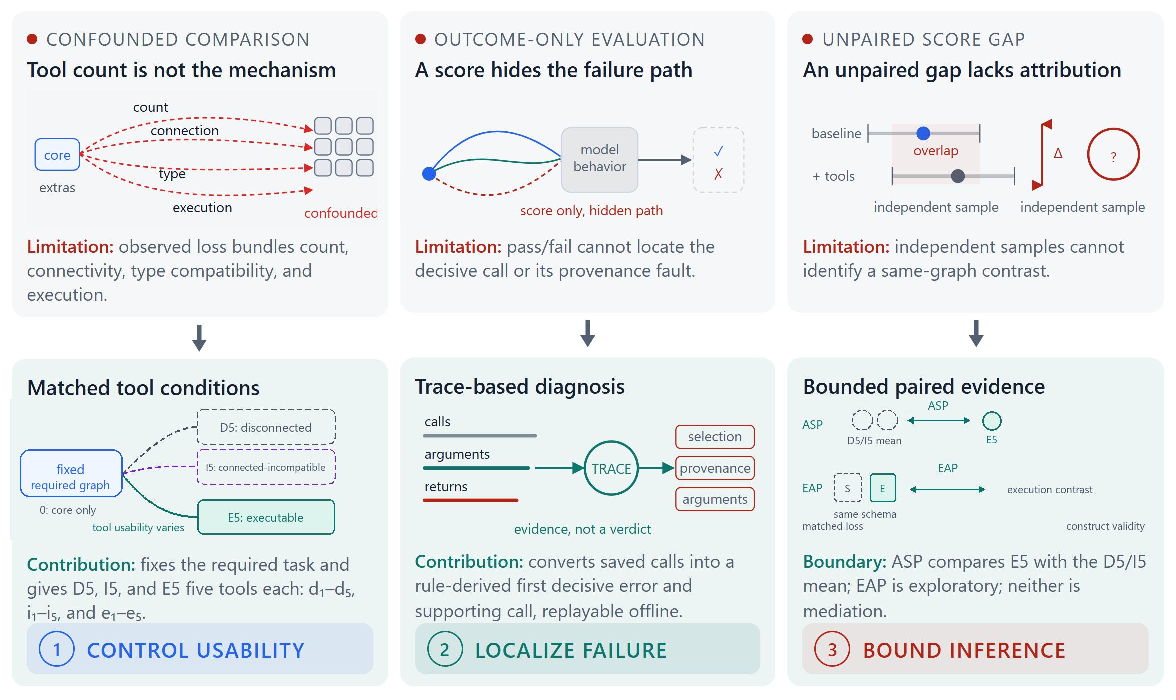
\includegraphics[width=\linewidth]{figure2_bottleneck_contributions_v0124.pdf}
\caption{\textbf{A3D links three evaluation gaps to one auditable workflow.}
The required dependency task is fixed before conditions are constructed.
Matched conditions vary the operational availability of extra branches; saved
calls are converted into a first-error diagnosis; and graph-matched summaries
separate outcome effects from mechanism claims. The figure labels
\emph{type-blocked} and \emph{runnable, off-goal} abbreviate connected-incompatible
and executable goal-irrelevant, respectively. Connectedness, type compatibility,
and runtime execution remain bundled in the main condition. ASP is a bounded
panel summary, and EAP is exploratory; neither is a causal mediation estimate.}
\label{fig:framework}
\end{figure}

Algorithm~\ref{alg:a3d} states the end-to-end procedure. Conditions are
constructed from the same required closure and are admitted only after invariant
audits. Model execution and diagnosis are intentionally separate: the execution
stage records tool calls, returned values, and errors, whereas the diagnostic
stage can later reproduce the report without another provider call.

\begin{algorithm}[htbp]
\caption{A3D matched diagnosis}
\label{alg:a3d}
\begin{algorithmic}[1]
\Require Graph seed \(s\), condition set \(\mathcal C\), model alias \(m\),
and inference configuration \(\theta\)
\Ensure Verified outcomes, saved traces, reports identifying the first decisive
error, and effect estimates
\State Generate the required graph \(G_s\), target closure \(R_s\), and target
truth \(y_s\)
\For{each condition \(c\in\mathcal C\)}
  \State Construct tool condition \(W_{s,c}\) from the fixed task and
  extra-tool condition \(c\)
  \State Audit full and required-graph fingerprints, target truth, prompts, and
  core order
  \State Execute model \(m\) with configuration \(\theta\) and save all calls,
  arguments, returned values, errors, and the final answer
  \State Compute the exact success rate and technical/budget-failure status
  \State Identify the first decisive error, record the supporting call, and
  produce a structured report
\EndFor
\State Estimate paired condition contrasts, ASP, and schema-matched EAP only on
verified shared graphs
\State Return the paired outcomes, diagnoses, effect estimates, and audit record
\end{algorithmic}
\end{algorithm}

\subsection{Audit system contract}

A3D is used here as a diagnostic system rather than as a claim that a new agent
architecture improves task success. Its input is a set of paired trials with a
fixed graph seed, condition label, model configuration, prompt, core tool order,
target truth, and saved call trace. Its admission checks are the required
fingerprint, prompt and target invariants, and a valid completed execution or an
explicit technical failure. Its outputs are the exact-success label, the
rule-derived first decisive error, the missing and irrelevant functions, trace
metrics, a diagnostic explanation, and an engineering check suggested by that
diagnosis. All outputs can be regenerated from the released trial record without
contacting a model provider.

\subsection{Required-graph invariants}

For each graph seed, a core dependency graph is generated and fixed. The target
variable, target truth, input variables, prompt, and core tool order are shared
between paired conditions. Connected extra tools add nodes and edges outside the
required closure. Consequently, ``same graph'' in this paper means the same
required dependency subgraph and task, not a visually identical tool set.

The audit records a full graph fingerprint and a required-graph fingerprint.
The required fingerprint covers the target closure and the audited task
invariants. A completed run with mixed graph generation across processes is not
admissible. Sorting set-derived structure before construction makes generation
repeatable across Python hash seeds.

This check changes the interpretation of a benchmark comparison. A model-level
score can be attributed to the added extra-tool condition only if the paired
task, target, and required closure are unchanged. The audit is part of the data
artifact, not a post-hoc narrative.

The invariant layer turns ``same graph'' from a descriptive claim into a
reproducible admission criterion, so an invalid mixed-generation run cannot
silently enter the paired analysis.

\subsection{Operational-availability conditions}

We distinguish four data conditions:
\begin{itemize}
\item \emph{none}: no intermediate extra tools are added;
\item \emph{disconnected}: five visible tools are added without a route from
the current state and without an executable input;
\item \emph{connected-incompatible}: five tools are structurally connected but
require an unavailable input type or value;
\item \emph{executable goal-irrelevant}: five tools are connected and have
type-compatible inputs, so an irrelevant branch can execute.
\end{itemize}

Each core task exposes four required tools. The \emph{none} condition therefore
contains four visible tools. Each five-tool condition adds five tools to the same
required closure, yielding nine visible tools. The modes differ in connectivity,
type availability, and executability while preserving the required task, target,
and core order. This does not fully factor every graph property, but it
addresses the simplest alternative explanation that the number of exposed tools
alone drives the result.

The tool-usability condition layer keeps the required task fixed and makes the
remaining ambiguity explicit. A positive contrast therefore supports a
condition-specific interpretation without claiming that connectivity, type
compatibility, and execution can be separated in every observed case.

\subsection{First-error diagnosis}

For each trial, A3D computes required-function recall, selection precision,
dependency-order score, argument score, and their equal-weight mean. It records
calls, arguments, returned values, tool errors, and the final answer. The
primary failure rule follows a fixed priority:
\begin{enumerate}
\item technical or budget failure when no usable trajectory exists;
\item premature final answer when the model stops before computing the target;
\item unknown function, premature dependency, or wrong argument value when the
corresponding call evidence is present;
\item irrelevant function when a non-required branch is executed;
\item incomplete chain when required functions are absent;
\item final-answer error when the required calls exist but the target does not
match.
\end{enumerate}

The report identifies the earliest call supporting the primary category,
lists missing and irrelevant functions, and recommends a concrete check. For
example, an irrelevant-function-call report recommends comparing every selected
function with the target closure and testing whether a type-compatible tool
became executable. The diagnosis is rule-derived; no human inter-rater study is
included. Its immediate claim is therefore auditability, not agreement with a
human's interpretation of model intent. Every label remains traceable to a
specific call, argument, returned value, or error.

The trace-evidence layer turns a binary outcome into an audit path anchored at
the first decisive error. A developer can use it to distinguish selection,
provenance, ordering, and premature-final failures before changing the system.

\subsection{Matched outcome summaries}

The primary outcome is the exact success rate. We report both model-specific
contrasts and a fixed-panel summary. The panel summary is descriptive: it treats
the five evaluated aliases as the study panel and does not estimate a
distribution of models. For the main comparison, define the paired change for
model \(m\) on graph \(g\) as

\begin{equation}
d_{g,m}=Y_{5,g,m}-Y_{0,g,m},
\qquad
\Delta_{\mathrm{study}}
=\frac{1}{G}\sum_{g=1}^{G}\frac{1}{M}\sum_{m=1}^{M}d_{g,m}.
\label{eq:study-main}
\end{equation}

We summarize \(\Delta_{\mathrm{study}}\) by resampling graph clusters and by a
two-sided graph-cluster sign-flip test. Resampling graphs preserves the sharing
of each graph across model aliases; the test does not treat the
\StudyMainPairs{} model-graph rows as independent. The model-specific deltas and
their McNemar results remain secondary analyses.

For each graph, the two five-tool controls provide a natural comparison for the
executable goal-irrelevant condition. Let
\(Y_D,Y_I,Y_{GI}\in\{0,1\}\) denote exact success outcomes with five
disconnected tools, five connected-incompatible tools, and five executable
goal-irrelevant tools,
respectively. The per-graph score and model-level ASP are

\begin{equation}
a_{m,g}=\frac{Y_D+Y_I}{2}-Y_{GI},
\qquad
\operatorname{ASP}_m
=100\,\mathbb{E}_g[a_{m,g}].
\label{eq:asp}
\end{equation}

ASP, the Affordance-Specific Penalty retained as a historical name, is measured
in percentage points. A positive value means that the
executable goal-irrelevant condition has a lower exact success rate than the average of the two
equal-count controls. The two differences are also reported separately so that
the average does not hide which control drives the result. The fixed-panel
summary is

\begin{equation}
\operatorname{ASP}_{\mathrm{study}}
=\frac{1}{G}\sum_{g=1}^{G}\frac{1}{M}\sum_{m=1}^{M}a_{m,g}.
\label{eq:asp-study}
\end{equation}

The sealed probe asks a narrower question: does runtime execution matter when
tool names, descriptions, JSON schemas, order, prompt, graph, and target are
identical? Let \(Y_E\) and \(Y_S\) denote exact success outcomes with executable and
sealed tools. The EAP is

\begin{equation}
\operatorname{EAP}_m
=100\,\mathbb{E}_g[Y_S-Y_E].
\label{eq:eap}
\end{equation}

A positive Executable-Affordance Penalty (EAP), like ASP retained as a historical
name, means that the model does better when the same executable goal-irrelevant
tools cannot execute. The probe uses 10 graphs and is treated as exploratory
construct-validity evidence.

\subsection{Offline use}

Diagnosis is separated from model execution. A saved run can therefore be
re-audited after the rules change, and a report can be checked without provider
access or a new model sample. The supplementary material contains the command
line interface and the complete report format. Legacy filenames and fields
retain historical identifiers such as ``affordance'' and
``connected\_compatible'' for reproducibility; they are not reader-facing
definitions of tool usability.

\section{Experimental Design}

Table~\ref{tab:design} summarizes the graph clusters, conditions, models, and
condition-level attempt counts used in the main comparison and supporting
studies. Graph clusters recur across studies; reused conditions and cells are
not additional independent tasks.

\begin{table}[htbp]
\centering
\caption{The main comparison and supporting studies use the same five models. Reused baseline cells are not additional independent tasks.}
\label{tab:design}
\footnotesize
\setlength{\tabcolsep}{3pt}
\renewcommand{\arraystretch}{1.08}
\begin{tabularx}{\textwidth}{>{\raggedright\arraybackslash}Xr>{\raggedright\arraybackslash}Xrr}
\toprule
Study & Graph clusters & Conditions & Models & Condition-level attempts \\
\midrule
Main & 20 & 0 / 5 executable goal-irrelevant & 5 & 200 \\
Dose & 15 & 0 / 2 / 5 executable goal-irrelevant & 5 & 225 \\
Controls & 15 & 0 / disconnected / connected-incompatible / executable goal-irrelevant & 5 & 300 \\
Prerequisite hiding & 8 & unhidden / hidden & 5 & 80 \\
Reminder & 4 & base / reminder & 5 & 40 \\
Repeatability & 8 & 0 / 5 executable goal-irrelevant & 5 & 80 \\
Sealed probe & 10 & executable / sealed & 5 & 100 \\
\bottomrule
\end{tabularx}
\par\parbox{\linewidth}{\raggedright\footnotesize Source: \texttt{configs/\allowbreak{}funcbench\_*.yaml}.}
\par\parbox{\linewidth}{\raggedright\footnotesize All five model aliases are evaluated in every study. Graph clusters recur across studies; reused conditions and cells are not additional independent tasks.}
\end{table}


\subsection{Models and API configuration}

We evaluated DeepSeek Flash, Kimi K3.1 Pro, GLM-5.3-Flashx,
MiniMax-M3.1-Flash, and Qwen3.8-Max on 2026-10-29, 2026-10-30, and
2026-11-01. The models were invoked through
direct provider endpoints with \texttt{trust\_env=false}. The shared
configuration used temperature 1.0, top-p 0.95, a maximum of 8192 output tokens,
low reasoning effort where supported, a 300-second timeout, and at most two
retries. MiniMax-M3.1-Flash does not allow thinking to be disabled; we used its
lowest supported effort and preserved returned reasoning content across tool
turns.

Service aliases are not immutable model snapshots. We therefore report the
endpoint alias, configuration snapshot, and execution date rather than treating
a provider name as a permanent model version.

\subsection{Units, conditions, and sample sizes}

The main experiment contains 20 independent depth-three graph clusters, two
endpoint conditions, and five models, producing 200 attempts. The last five
graphs extend the first 15. The dose study uses 15 shared graphs at 0, 2, and 5
executable goal-irrelevant tools, producing 225 condition-level attempts.

The graph cluster is the independent design unit. A condition-level attempt is a
repeated model evaluation within that unit, and the same graph contributes rows
for several model aliases. Consequently, the 200 main attempts do not represent
200 independent tasks, and the five model-specific results do not represent five
independent populations. All inferential summaries preserve the graph-cluster
pairing.

The tool-usability control uses 15 shared graphs in four modes, producing 300
attempts. The prerequisite-hiding intervention compares unhidden and hidden
executable goal-irrelevant runs on eight graphs, producing 80 attempts. The state
reminder uses four graph-matched pairs, producing 40 attempts. Baseline cells
are reused across analyses; the condition-level counts are not additive
independent task counts.

The schema-matched sealed probe uses 10 shared graphs and two conditions,
producing 100 condition-level attempts. Its executable cells reuse the main
executable goal-irrelevant results; the 50 sealed trials are new.

A separate repeatability run uses the same eight graph indices and generator
seed as the original first-eight subset, but makes fresh model calls. It adds
80 attempts and covers zero and five executable goal-irrelevant tools for all
five models.

\subsection{Outcomes and statistics}

Exact success is the primary outcome. A trial is correct only when the final
answer matches the program-computed target. Technical/budget failures remain failures
in the main analysis and are separately reported for sensitivity.

As a secondary, post-hoc descriptive summary, we report the mean paired change
in Equation~\ref{eq:study-main}. This summary was defined after the
model-specific analyses and is not a pre-specified confirmatory endpoint. Its
interval resamples graph clusters, and its two-sided sign-flip test assigns one
sign to every model contrast sharing the same graph. The test describes whether
the panel-level contrast is unusual under exchangeable graph signs; it does not
estimate a random-effects distribution across models. The model-specific paired
bootstrap intervals and exact McNemar tests answer the separate question of
whether any individual model has effect after multiplicity control. Failure to
clear that stricter hurdle is not treated as absence of a panel-level
association.

No a priori precision target was set for the 20-graph panel. The observed
graph-cluster interval is therefore reported as a descriptive precision
statement rather than as confirmation of a powered design.

For ASP and EAP, intervals also resample graphs and two-sided sign-flip tests
use graph-level scores. The fixed-panel ASP is defined in
Equation~\ref{eq:asp-study}; model-level ASP and EAP remain secondary, with Holm
adjustment reported across the five aliases. The bootstrap and sign-flip
procedures use a fixed deterministic seed in the asset builder.

\section{Results}

\subsection{Executable goal-irrelevant tools are associated with lower exact success rates}

\begin{table}[htbp]
\centering
\caption{Five executable goal-irrelevant tools were associated with a paired loss in the exact success rate in every model.}
\label{tab:main20}
\footnotesize
\setlength{\tabcolsep}{3pt}
\renewcommand{\arraystretch}{1.08}
\begin{tabularx}{\textwidth}{>{\raggedright\arraybackslash}Xrrrrr}
\toprule
Model & 0 extra tools & 5 goal-irrelevant & Delta [95\% CI] & Exact McNemar p & Holm p \\
\midrule
DeepSeek & 20/20 (100.0\%) & 14/20 (70.0\%) & -30.0 pp [-50.0, -10.0] & 0.0312 & 0.1250 \\
Kimi & 13/20 (65.0\%) & 7/20 (35.0\%) & -30.0 pp [-55.0, -5.0] & 0.0703 & 0.2109 \\
GLM & 7/20 (35.0\%) & 5/20 (25.0\%) & -10.0 pp [-35.0, +15.0] & 0.6875 & 0.6875 \\
MiniMax & 16/20 (80.0\%) & 8/20 (40.0\%) & -40.0 pp [-65.0, -15.0] & 0.0215 & 0.1074 \\
Qwen & 17/20 (85.0\%) & 11/20 (55.0\%) & -30.0 pp [-60.0, -5.0] & 0.1094 & 0.2188 \\
\bottomrule
\end{tabularx}
\par\parbox{\linewidth}{\raggedright\footnotesize Source: \texttt{results/\allowbreak{}funcbench-main20-five-model-analysis-20261101/\allowbreak{}paired\_effect\_summary.csv}.}
\par\parbox{\linewidth}{\raggedright\footnotesize Each model has 20 paired graphs. Intervals are paired graph-level bootstrap intervals. McNemar tests are uncorrected in the source file; Holm values are derived here.}
\end{table}


Table~\ref{tab:main20} and Figure~\ref{fig:core-evidence} show the same paired
pattern. As a secondary descriptive summary, exact success changed across the
fixed panel from
\StudyMainBaseCorrect/\StudyMainPairs{} to
\StudyMainDistCorrect/\StudyMainPairs{}, a mean paired loss of
\StudyMainDeltaPP{} points (graph-cluster 95\% CI
[\StudyMainCILowPP, \StudyMainCIHighPP]; sign-flip p=\StudyMainSignFlipP).
Of the \StudyMainPairs{} paired model-graph comparisons,
\StudyBaselineOnly{} moved from correct to incorrect and
\StudyDistractorOnly{} moved in the opposite direction.
\StudyMainNegativeGraphs{} of the 20 graph-level mean deltas were negative,
\StudyMainZeroGraphs{} were zero, and \StudyMainPositiveGraphs{} were positive.

At the model level, every point estimate was negative and ranged from 10 to 40
percentage points. The graph-bootstrap interval excluded zero for every model
except GLM, and the uncorrected exact McNemar tests ranged from
\DeepSeekMcNemarP{} to \GLMMcNemarP. No test remained below 0.05 after Holm
correction. The panel summary and the model-level tests therefore answer
different questions: the former describes a consistent direction across this
fixed panel, whereas the latter apply a stricter multiplicity guard to separate
model-level claims.

\begin{figure}[htbp]
\centering
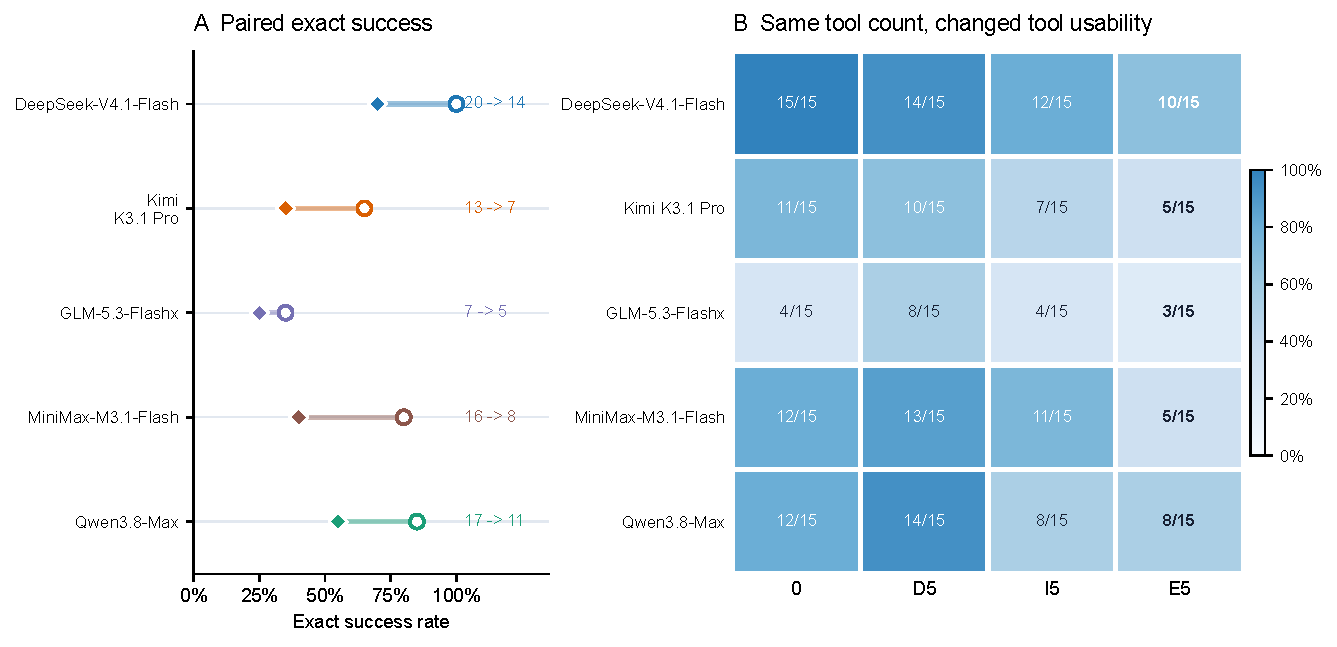
\includegraphics[width=\linewidth]{figure3_core_evidence.pdf}
\caption{\textbf{The lowest exact success occurs when the extra tools can
execute.} Panel A shows paired exact success rates on 20 shared graphs; each pair is
0 versus 5 executable goal-irrelevant tools. Panel B holds the number of extra
tools at five on 15 shared graphs. Executable goal-irrelevant tools are lowest or tied
for lowest in every model. In Panel B, D5, I5, and E5 denote the disconnected,
connected-incompatible, and executable goal-irrelevant conditions with five added
tools.}
\label{fig:core-evidence}
\end{figure}

The model ordering was DeepSeek $>$ Qwen $>$ MiniMax $>$ Kimi $>$ GLM in both
main conditions, with no reversal. The graph-cluster permutation test for an
interaction gave p=\InteractionP{} and a \InteractionEffectRangePP-point range
among paired effects, so the data do not show statistically different
model-specific effects. One DeepSeek trial produced an empty response under
five extra tools; excluding it changes success from 14/20 to 14/19 and leaves
the direction unchanged.

\subsection{The loss is not explained by tool count alone}

The equal-count comparison addresses the main alternative explanation. On 15
shared graphs, disconnected tools did not reproduce the executable goal-irrelevant
condition's loss, and connected-incompatible tools did not produce a stable
similar loss. The executable goal-irrelevant condition was lowest for DeepSeek, Kimi,
GLM, and MiniMax, and tied with the connected-incompatible condition for Qwen.
The disconnected condition had a higher exact success rate than the executable goal-irrelevant condition
for every model.

If tool count were the main mechanism, adding five disconnected tools should
produce a similar loss. That pattern does not appear, so the result cannot be
explained by count alone.

ASP was positive for all five models, ranging from \ASPRangeLowPP{} to
\ASPRangeHighPP{} points. The fixed-panel summary was
\StudyASPP{} points (graph-cluster 95\% CI
[\StudyASPCILowPP, \StudyASPCIHighPP]; sign-flip p=\StudyASPSignFlipP).
The graph-level averages were positive in \StudyASPPositiveGraphs{} graphs, zero
in \StudyASPZeroGraphs{}, and negative in \StudyASPNegativeGraphs{}. Only MiniMax
survived model-level Holm correction (\MiniMaxASPHolmP; bootstrap 95\% CI
[\MiniMaxASPLowPP, \MiniMaxASPHighPP]). Figure~\ref{fig:asp} shows the model
estimates and their relation to success without extra tools. The panel direction
is consistent; the evidence still does not support a model ranking or a claim
that the three bundled properties have separate causal effects.

\begin{figure}[htbp]
\centering
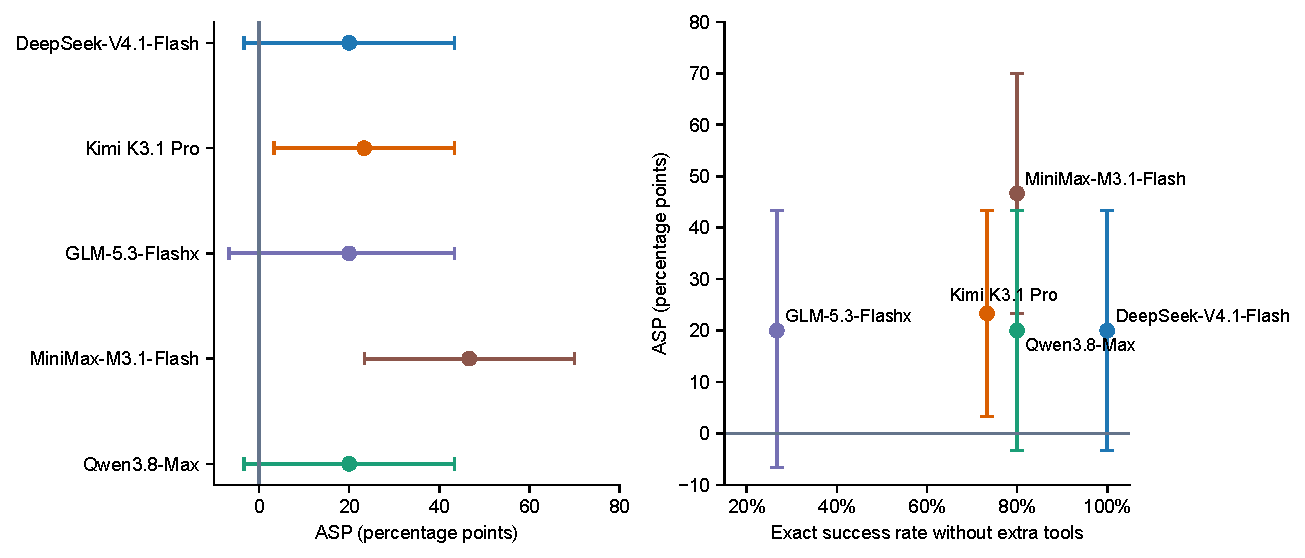
\includegraphics[width=\linewidth]{figure4_asp.pdf}
\caption{\textbf{Executable goal-irrelevant tools show positive paired losses in every
model.} Left: graph-bootstrap intervals for ASP against zero. Right: ASP
relative to the exact success rate with no extra tools. Only MiniMax remains below 0.05
after Holm correction.}
\label{fig:asp}
\end{figure}

The restricted analysis on graphs solved without extra tools gives the same
cautious picture and is reported in the supplement. MiniMax retained a positive
estimate, but no restricted ASP survived five-model Holm correction. Small
solvable subsets, especially for GLM, make this a sensitivity analysis rather
than a stable model property.

\subsection{The executable branch changes the first-error mix}

The final score hides very different trajectories. Across the 200 main trials,
118 were correct, 23 had a wrong argument value, 29 showed premature dependency
use, 22 made an irrelevant function call, seven gave a premature final answer,
and one had a technical/budget failure. With zero extra tools, no trial made an
irrelevant function call or gave a premature final answer. With five extra tools,
22 made an irrelevant function call and seven gave a premature final answer.

If the final score captured the whole failure process, the set of first
decisive error categories would not change when the tool environment changes.
The observed shift shows that the trace adds information about where the task
went wrong.

Figure~\ref{fig:errors} shows that these totals come from different
model-specific mixtures. This is why the paper treats trace evidence as a
diagnostic result rather than as a replacement for the exact success rate. A saved
DeepSeek trajectory provides a concrete example: the model spent its action
budget on an executable goal-irrelevant tool. Other trajectories show wrong argument
values, premature dependency use, or premature final answers. The complete
reports are in the
supplement; the labels are deterministic rules rather than human-validated
categories.

\begin{figure}[htbp]
\centering
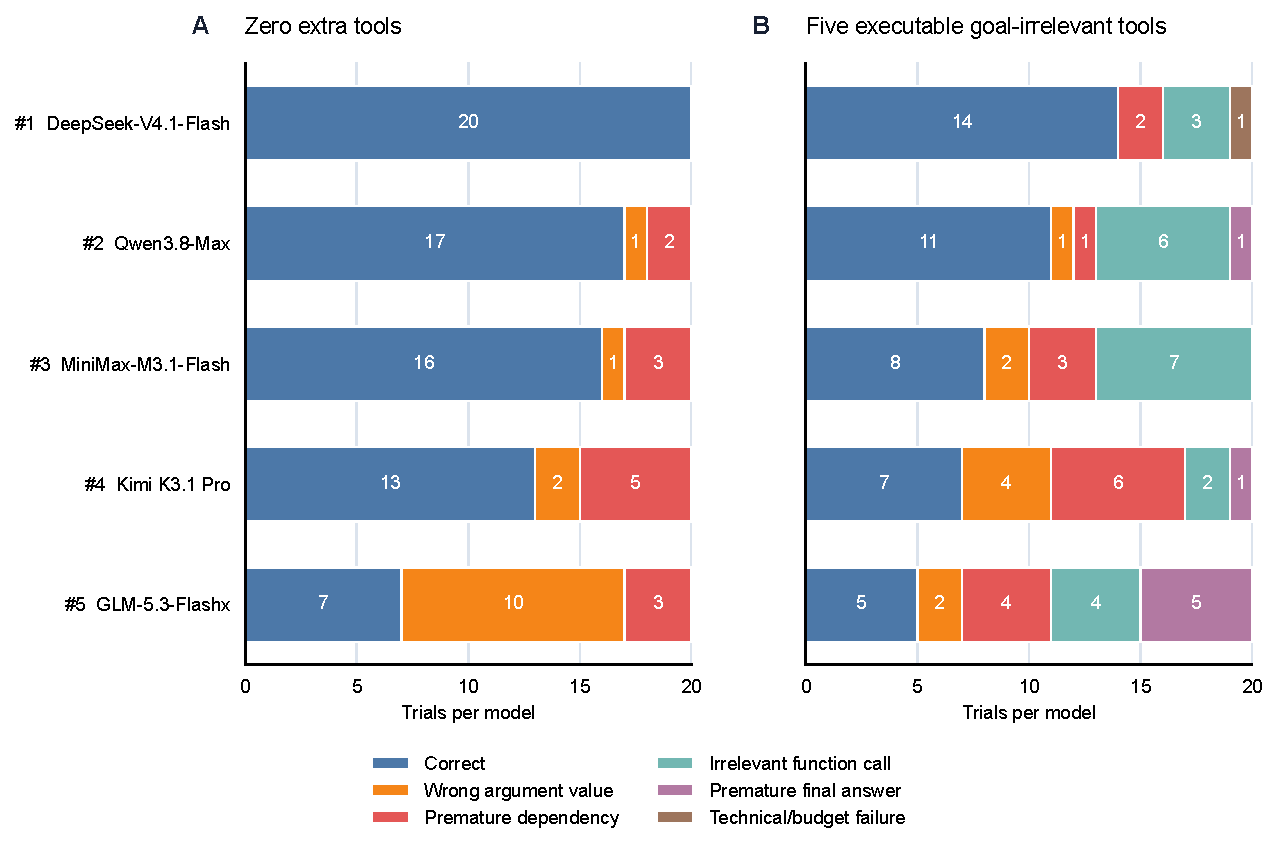
\includegraphics[width=\linewidth]{figure6_errors.pdf}
\caption{\textbf{An executable branch changes how tasks fail.} Rule-derived
primary outcomes are shown for zero and five executable goal-irrelevant tools.
Each bar contains 20 trials. Irrelevant function calls and premature final
answers appear only in the five-extra-tool condition.}
\label{fig:errors}
\end{figure}

\subsection{Execution is directionally implicated, but the probe is exploratory}

The schema-matched sealed probe changes only runtime execution. The model sees
the same tool names, descriptions, JSON schemas, order, prompt, graph, and
target in both conditions. Sealing the executable goal-irrelevant tools increased
the exact success rate for four models and left Kimi unchanged: EAP was 20.0
points for DeepSeek, 0.0 for Kimi, 40.0 for GLM, 40.0 for MiniMax, and 20.0 for
Qwen.

Figure~\ref{fig:sealed} shows the condition rates and intervals. GLM and
MiniMax had bootstrap intervals excluding zero, but their sign-flip p-value was
0.125, and no model survived Holm correction. The result therefore supports
execution as a plausible part of the failure process without establishing it as
the sole cause.

\begin{figure}[htbp]
\centering
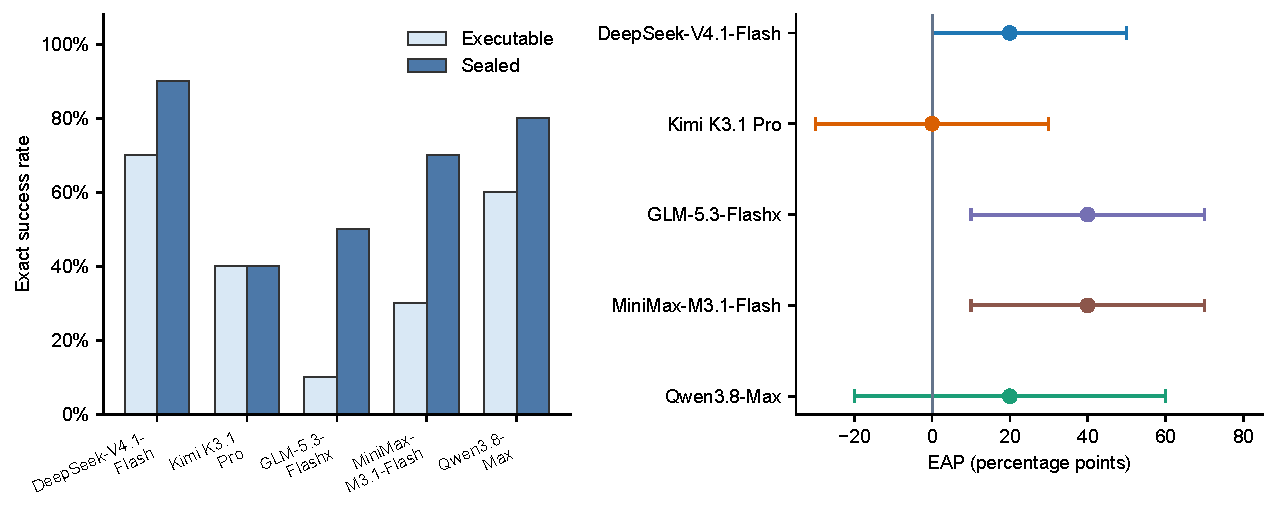
\includegraphics[width=\linewidth]{figure5_sealed.pdf}
\caption{\textbf{Blocking execution improves success for four models, but not
strongly enough for a corrected model-level claim.} The executable and sealed
conditions use identical tools and schemas; only whether a tool can run
changes. The 10-graph probe is exploratory.}
\label{fig:sealed}
\end{figure}

\subsection{Stability and simple interventions}

The conclusions are not equally stable across models. A fresh sample on eight
graphs reproduced 67/80 correctness labels (83.75\%; Cohen's kappa 0.673). The
executable-goal-irrelevant-condition decline repeated for DeepSeek, Kimi, MiniMax, and Qwen;
GLM remained near its low baseline and did not repeat it.

Two attempts to support the model produced no net improvement. A state reminder
on four shared graphs left one model worse and four unchanged. On eight shared
graphs, prerequisite hiding reduced success for all five models. These results
argue against treating either a generic reminder or the removal of
not-yet-available tools as a reliable repair. A 0/2/5 pattern and the full
intervention tables are reported in the supplement; they support no common
linear threshold.

\section{Diagnostic Validity and Applied Use}

The claim supported by the trace layer is bounded by the evidence available for
the labels. Primary categories are assigned by fixed rules in the order:
technical or budget failure; premature final answer; unknown function,
premature dependency, or wrong argument value when the corresponding call
evidence exists; irrelevant function; incomplete chain; and final-answer error.
The first matching rule supplies one primary category, and the report retains
the originating call. This procedure makes diagnoses reproducible and
inspectable, but it does not establish human inter-rater agreement or recover an
unobserved model intention.

For applied use, the report is therefore best understood as a pre-deployment
audit. An \emph{irrelevant-function} diagnosis directs the developer to inspect
whether a connected and executable off-goal branch is present. A
\emph{premature-dependency} diagnosis directs attention to state provenance. A
\emph{wrong-argument} diagnosis points to value construction. A
\emph{premature-final} diagnosis points to termination conditions. These are
checks suggested by observable evidence, not causal findings about why the
model generated the action.

An illustrative offline workflow makes the intended use concrete without adding
an effectiveness claim:
\begin{enumerate}
\item select a failed saved trial whose required-graph audit passed;
\item read the reported primary category and first decisive call;
\item inspect the indicated selection, provenance, argument, or termination
  evidence;
\item compare the same graph and condition after a candidate scaffold change,
  while keeping exact success as the primary outcome;
\item preserve the report as run-local evidence rather than promoting it to a
  safety verdict.
\end{enumerate}
This workflow shows how a deterministic report can organize an engineering
review. It does not show that using A3D improves a developer's decision or the
system's success rate.

The system also separates execution from audit. A saved trial record can be
reanalysed after the diagnostic rules are inspected, without another provider
call. This is useful when reviewing a single failure, comparing a changed agent
scaffold on the same graph, or deciding which trace field must be instrumented
more carefully. It does not make A3D a production safety certificate: the rule
labels remain heuristic, the provider aliases are not immutable snapshots, and
the audit covers one task family at depth three.

The deployment boundary is correspondingly narrow. Offline trace audit can
inspect saved evidence after a run; online gating would change the action space
and requires a separate paired evaluation; safety-critical deployment would
require validation, monitoring, and accountable human review beyond the present
study.

\section{Discussion}

\subsection{Implications for benchmark builders}

The equal-count controls change how benchmark difficulty should be described.
Two tasks that expose the same number of tools can pose different reliability
problems when their extra branches differ in connectivity, type availability,
and executability. A benchmark report should therefore state how many irrelevant
branches are present, how many can execute, and which required path each branch
competes with. The present design does not separate those three properties into
independent causal effects; it establishes that counting tools alone is an
incomplete description of the action space.

\subsection{Implications for agent and tool-schema developers}

Schema validation checks whether a call is possible. It does not check whether
the returned value advances the required dependency chain. A connected,
type-compatible executable goal-irrelevant tool can therefore pass every local
check and still make the trajectory invalid. The practical audit question is not
only whether a tool can be invoked, but whether its output has a valid role in
the current goal state. The first-error report makes that question inspectable
at the call that first changed the path.

\subsection{Why final success is not enough}

The trace results explain why a single success score cannot answer the question
that motivates the paper. Different models fail in different ways, and the
same model changes its dominant failure when an executable branch appears.
A3D reports the first decisive error and its supporting call because later
symptoms can be misleading: an invalid final answer may be preceded by an
irrelevant function call, a missing dependency, or a premature final answer.

This diagnostic view does not replace exact success. The outcome remains the
primary endpoint; the trace supplies the location to inspect when the endpoint
changes. The difference matters for applied debugging because a correct final
answer may follow an invalid intermediate branch, while an incorrect answer may
arise after earlier recovery attempts. The audit reports the earliest decisive
state change rather than assigning an unobserved intention to the model.

\subsection{Negative interventions define the application boundary}

Neither repeating the current state nor hiding unusable tools improved
success. Hiding tools also changes the action space, which can introduce new
failure paths. These negative results are consistent with the main finding:
making a branch unusable is not the same as helping the model decide which
usable tool is goal-relevant. They also limit the recommendation that can be
made from this study. A3D identifies where a system should intervene; it does
not establish that a particular intervention will improve reliability, and the
present evidence supports guided inspection rather than demonstrated decision
improvement. Learned or masking-based function-calling mitigations exist
\citep{lin2025hammer}; the present prerequisite-hiding result should not be
generalized to those different intervention mechanisms.

\section{Limitations}

The main analysis has 20 graph clusters, one temperature-1 sample per cell, one
task family, and five model aliases that are not immutable provider snapshots.
The fixed-panel summary is post-hoc and secondary; it addresses the direction
across these aliases but does not estimate a distribution of models or remove
sampling variation within a cell. No a priori precision target was set. The
repeatability audit covers eight graphs. The control and dose studies cover 15,
while the prerequisite-hiding and reminder studies cover eight and four. These
samples limit model-specific and interaction claims.

The core conditions still combine connectedness, type compatibility, and
execution. The execution probe narrows the gap but uses only 10 graphs and
produces no corrected model-level effect. Trace categories are deterministic
rules without independent human agreement; the audit claim is therefore
reproducibility and inspectability, not validated attribution. ASP and EAP are
descriptive paired losses, not causal mediation estimates. The study does not
establish a stable threshold, a general capability ranking, a production safety
certificate, or an effective repair.

\section{Conclusion}

An agent can fail after making calls that are individually valid. The missing
link is the required dependency path: an executable goal-irrelevant tool may run
successfully and still send an unusable value into the next step. A3D makes this
failure visible by holding the required task fixed, changing operational
availability without changing the number of added tools, and locating the first
decisive error in the saved trace.

Across the fixed five-model panel, executable goal-irrelevant tools were
associated with lower exact success than zero-tool and equal-count control
conditions. The secondary panel-level description was directionally clear, while
corrected model-level tests were limited. The practical conclusion is narrow:
schema validity and tool count are not enough to assess multi-step reliability.
Evaluation should also record which off-goal branches can execute, compare them
with equal-count controls, and retain first-error evidence from the execution
path.

\section*{Statements and Declarations}

\subsection*{Funding}
This work is jointly supported by NSFC (Grant No. 62366047) and the
Fundamental Research Funds for the Central Universities (Grant No. 31920240060).

\subsection*{Competing interests}
The author declares that there are no competing financial interests or
personal relationships that could have appeared to influence the work reported
in this paper.

\subsection*{Ethics approval and consent}
Not applicable. This study used synthetic function schemas and program-generated
tasks. It did not involve human participants, human tissue or personal data,
animals, or clinical interventions.

\subsection*{Consent for publication}
Not applicable.

\subsection*{Originality and prior publication}
This manuscript is original, has not been published previously in whole or in
part, and is not under consideration for publication elsewhere.

\subsection*{Data availability}
The generated graph-condition data, configuration snapshots, sanitized
tool-call traces, trial-level outcomes, derived tables, and reproducibility
materials are publicly available at
\url{https://github.com/nywang2019/a3d-tool-audit}. The data release uses the
CC BY 4.0 license and contains no API keys, account tokens, credentials, or
personal request metadata. No separate archival DOI has been assigned.

\subsection*{Code availability}
The source code for task and condition generation, model execution, graph
invariant auditing, first-error diagnosis, statistical analysis, and figure and
table reproduction is publicly available at
\url{https://github.com/nywang2019/a3d-tool-audit} under the MIT License.
Nianyi Wang is responsible for maintaining the archived release.

\subsection*{Author contributions}
Nianyi Wang: Conceptualization, Methodology, Software, Validation, Formal
analysis, Investigation, Data curation, Writing---original draft, Writing---review
and editing, Visualization, Project administration, Funding acquisition.

\subsection*{Use of AI}
OpenAI Codex was used as a non-author AI research assistant during manuscript
preparation. Its contribution included manuscript restructuring and adversarial
questioning, consistency audits of the text against figures, tables, and source
data, literature-positioning checks, LaTeX editing and build verification, and
packaging of the public reproducibility artifact. Codex did not generate the
empirical results, perform model trials, substitute for independent peer review,
or take responsibility for the work. Nianyi Wang directed the work, verified all
AI-assisted outputs, approved the scientific claims, and accepts full
responsibility for the manuscript and released materials.

\footnotesize
\bibliography{references}

\end{document}

